\documentclass[handout]{beamer}

\usepackage[utf8]{inputenc} % Language and font encoding
\usepackage[icelandic]{babel}
\usepackage[T1]{fontenc}


\usepackage{tikz}
\usepackage[listings,theorems]{tcolorbox}
\usepackage{booktabs}
\usepackage{minted} %Minted and configuration
\usemintedstyle{default}

\renewcommand{\theFancyVerbLine}{\sffamily \arabic{FancyVerbLine}}
%%%%%%%%%%%
% More math
%%%%%%%%%%%
\newcommand{\Mod}[1]{\ \text{mod}\ #1}

%%%%%%%%%%%%%%%%%%%%%%
% Beamer configuration
%%%%%%%%%%%%%%%%%%%%%%
\setbeamertemplate{navigation symbols}{}
\usecolortheme{dove}
\setbeamercolor{frametitle}{fg=white}

\usebackgroundtemplate%
{%
\vbox to \paperheight{

\includegraphics[width=\paperwidth]{Pics/hi-slide-head-2016}

\vfill
\hspace{0.5cm}
\includegraphics[width=0.3\paperwidth]{Pics/hi-von-logo}
\vspace{0.4cm}
    }%
}

\AtBeginSection[]
{
  \begin{frame}<beamer>
    \frametitle{Yfirlit}
    \tableofcontents[currentsection]
  \end{frame}
}

\setbeamerfont{frametitle}{size=\normalsize}
\addtobeamertemplate{frametitle}{}{\vspace*{0.5cm}}

%%%%%%%%%%%%%%%%%%%%%%%%%
% tcolorbox configuration
%%%%%%%%%%%%%%%%%%%%%%%%%

% Setup from: http://tex.stackexchange.com/a/43329/21638
\tcbset{%
    noparskip,
    colback=gray!10, %background color of the box
    colframe=gray!40, %color of frame and title background
    coltext=black, %color of body text
    coltitle=black, %color of title text 
    fonttitle=\bfseries,
    alerted/.style={coltitle=red, colframe=gray!40},
    example/.style={coltitle=black, colframe=green!20, colback=green!5},
}


%%%%%%%%%%%%%%%%%%%%%%%
% Further configuration
%%%%%%%%%%%%%%%%%%%%%%%
\hypersetup{colorlinks=true,pdfauthor={Eirikur Ernir Thorsteinsson},linkcolor=blue,urlcolor=blue}
\graphicspath{{./Pics/}}

\author{Eiríkur Ernir Þorsteinsson}
\institute{Háskóli Íslands}
\date{Haust 2016}

\title{Tölvunarfræði 1a}
\subtitle{Vika 1, fyrri fyrirlestur}

\begin{document}

\begin{frame}
\titlepage
\end{frame}

\section{Um námskeiðið}

\begin{frame}{Kennari}
\begin{columns}
\column{0.5\textwidth}
\begin{itemize}
 \item Nafn: Eiríkur Ernir Þorsteinsson
 \item Aðsetur: Tæknigarði, 2. hæð, herbergi 214
 \item Tölvupóstfang: \href{mailto:eth31@hi.is}{eth31@hi.is}
 \begin{itemize}
  \item Sjá einnig: \hyperlink{frame:piazza}{Piazza}
 \end{itemize}
\end{itemize}
\column{0.5\textwidth}
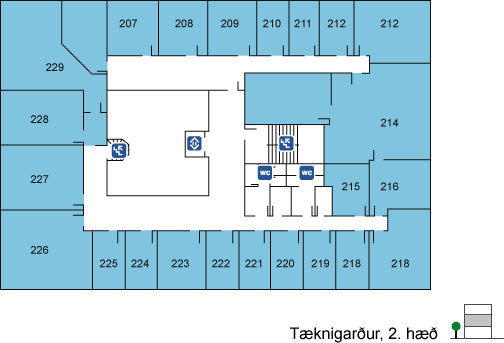
\includegraphics[width=\linewidth]{taeknigardur}
\end{columns}
\end{frame}

\begin{frame}{Tímar}
\begin{itemize}
 \item Fyrirlestrar
 \begin{itemize}
  \item Miðvikudögum klukkan 8:20 í VRII 158, föstudögum klukkan 11:40 í VRII 157
  \item Fyrirlestrar fara hratt yfir efni kennslubókarinnar
 \end{itemize}
 \item Dæmatímar
 \begin{itemize}
  \item Hefjast í næstu viku
  \item Farið stuttlega yfir skil síðustu viku, nokkur tímaverkefni (sem dæmatímakennarar hjálpa við)
  \item Þrír hópar, seint á mánudögum og þriðjudögum
  \begin{itemize}
   \item Einungis þarf að mæta í \emph{einn}
  \end{itemize}
  \item Hópum verður úthlutað fljótlega\textsuperscript{\textregistered}
 \end{itemize}
\end{itemize} 
\end{frame}

\begin{frame}{Námsmat}
\begin{itemize}
 \item Vikuleg heimaverkefnaskil
 \begin{itemize}
  \item Gilda 20\% samtals
  \item 10 bestu verkefni gilda til einkunnar
  \item \emph{Skila þarf 5 af fyrstu 7 heimaverkefnunum til að öðlast próftökurétt}
 \end{itemize}
 \item Fyrirlestraæfingar
 \begin{itemize}
  \item Gilda 10\% samtals
  \item 20 skil gefa fulla einkunn
  \item Tekið er tillit til fjarnema og fólks í árekstrum (hafið samband!)
 \end{itemize}
 \item Miðmisserispróf (líklega laugardaginn 17. október)
 \begin{itemize}
  \item Gildir 20\% ef það leiðir til hækkunar, annars 0\%
 \end{itemize}
 \item Lokapróf
 \begin{itemize}
  \item Gildir 50\% ef miðmisserispróf leiðir til hækkunar, annars 70\%
  \item Lágmarkseinkunn á prófi og námskeiðinu í heild er 5.
 \end{itemize}
\end{itemize}
\end{frame}

\begin{frame}{Álag}
Námskeiðið er $6 ECTS$ einingar. 60 ECTS einingar eru skilgreindar sem 1500-1800 klst. af vinnu.
\[
\text{60 ECTS = 1650 klst.} \Longleftrightarrow \text{6 ECTS = 165 klst.}
\]
Misserið er 14 vikur, svo gera má ráð fyrir 11-12 klst. af vinnu í hverri viku. Þar af eru 4 klst. í fyrirlestrum og dæmatímum.
\end{frame}

\subsection{Námefni og tól}

\begin{frame}{Bók}
\begin{columns}
\column{0.5\textwidth}
Aðalbók:
\begin{center}
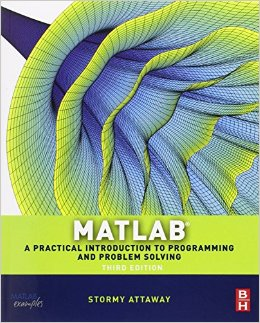
\includegraphics[width=0.66\linewidth]{Pics/matlab_stormy}
\end{center}
Þessari bók verður fylgt nokkuð vandlega \pause
\column{0.5\textwidth}
E.t.v. gagnleg til uppflettingar/hliðsjónar:
\begin{center}
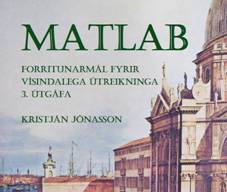
\includegraphics[width=0.7\linewidth]{Pics/matlab_kristjan}
\end{center}
Er á íslensku!
\end{columns}
\end{frame}

\begin{frame}{Verkefnaskil}
\begin{itemize}
 \item Verkefnaskil fara fram í vefkerfinu \href{https://gradescope.com/}{Gradescope}
 \begin{itemize}
  \item \url{https://gradescope.com/}
 \end{itemize}
 \item Aðgangskóði er \texttt{9WXZPM}
 \item Kerfið tekur við \texttt{.pdf} skrám
 \item Fyrstu skilin verða í næstu viku
\end{itemize}
\end{frame}

\begin{frame}{Fyrirspurnir og umræður}
\label{frame:piazza}
\begin{itemize}
 \item Spjallkerfið \href{piazza.com/hi.is/fall2016/tl105g}{Piazza} verður notað í þessu námskeiði
 \begin{itemize}
  \item \url{piazza.com/hi.is/fall2016/tl105g}
 \end{itemize}
 \item Kerfið mun vera besta leiðin til að fá svör frá samnemendum, dæmatímakennurum og undirrituðum
 \item Setjið allar fyrirspurnir um námskeiðið þangað!
 \begin{itemize}
  \item Kemur í stað tölvupósts
 \end{itemize}
\end{itemize}
\end{frame}

\begin{frame}{Fyrirlestraverkefni}
\begin{itemize}
 \item Í hverjum fyrirlestri verða lögð fyrir verkefni á vefnum \href{http://socrative.com/}{Socrative}
 \item Innskráningarferli:
 \begin{itemize}
  \item Notið ``herbergisnúmerið'' \texttt{TOL105G2016}
  \item Notendanafnið ykkar þarf að vera \textbf{HÍ-tölvupóstfangið ykkar}
  \begin{itemize}
   \item Passið að það sé rétt skrifað, annars finnist þið ekki!
  \end{itemize}
 \end{itemize}
 \item Þegar í herbergið er komið eigið þið að geta fundið þau verkefni sem sett hafa verið fyrir
\end{itemize}
\end{frame}

\subsection{Heilræði}

\begin{frame}{Heilræði}
\pause
\begin{itemize}
 \item Takið þátt í tímum\pause
 \begin{itemize}
  \item Réttið upp hönd, spyrjið! \pause
  \item Talið við dæmatímakennarana
 \end{itemize}
 \item Gerið dæmin \pause
 \begin{itemize}
  \item Færnin kemur í gegnum forritunaræfingar \pause
 \end{itemize}
 \item Nýtið aðstoð
 \begin{itemize}
  \item Dæmatímakennarar
  \item Samnemendur
  \item Námsráðgjöf HÍ \pause
 \end{itemize}
 \item Sofið og slakið á
\end{itemize}
\end{frame}

\section{Forritunarhugtakið}

\begin{frame}{Hvað er forritun?}
\pause
Sýn kennarans:
\begin{itemize}
  \item Tölvur eru fjölhæfar vélar
  \begin{itemize}
   \item Þær eru með margar mögulegar aðgerðir, svo þeim þarf að segja fyrir verkum
  \end{itemize}
  \item Það að forrita er að útskýra fyrir tölvunni hvað hún á að gera
  \item Þessar útskýringar eru á formi skipana
  \item Margar skipanir mynda saman forrit
  \item Vandamálið: Tölvur hugsa ekki
  \begin{itemize}
   \item Þær reikna.
   \item Þær skilja ekki.
   \item Þetta gerir samskipti við tölvur öðru vísi en samskipti fólks
  \end{itemize}
 \end{itemize}
\end{frame}

\begin{frame}{Forritunarmál}
\begin{itemize}
 \item Til þess að eiga samskipti við tölvu þurfum við að eiga sameiginlegt mál - forritunarmál
 \item Líkt og venjuleg tungumál hafa forritunarmál setningar- og málfræði (e. \emph{syntax}) ásamt merkingarfræði (e. \emph{semantics})
 \begin{itemize}
  \item Tölvur eru afar smámunasamar þegar kemur að syntax
  \item Það að geta komið merkingu til skila kemur með æfingu
 \end{itemize}
\end{itemize}
\end{frame}

\begin{frame}{Upplifunin}
\begin{center}
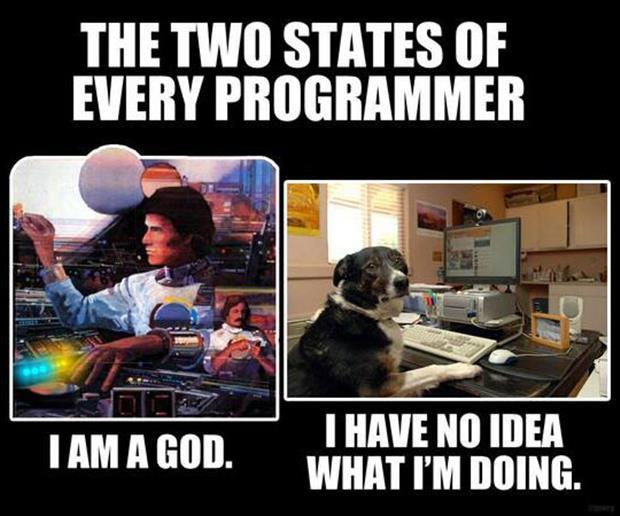
\includegraphics[height=0.85\textheight]{Pics/twostates} 
\end{center}
\end{frame}

\begin{frame}[fragile]{Forritunarmál - dæmi í Matlab}
Í Matlab-forritunarmálinu hefur skipunin
\begin{minted}[frame=lines]{matlab}
>> disp('Hello world!')
\end{minted}
merkinguna \emph{skrifaðu út orðin ``Hello world!''}.

\vspace{0.5cm}
Skipunin
\begin{minted}[frame=lines]{matlab}
>> 1+2;
\end{minted}
hefur merkinguna \emph{leggðu saman töluna 1 og töluna 2}.
\end{frame}

\section{Matlab}

\begin{frame}{Hvað er svo þetta Matlab?}
\begin{itemize}
 \item Matlab er a.m.k. tvennt:
 \begin{enumerate}
  \item \emph{Forritunarmál}, (m.a.) skilgreining á því hvernig setningarfræðin í ``samskiptamálinu'' er
  \item \emph{Forritunarumhverfi}, forrit sem (m.a.) tekur við skipununum frá notandanum og túlkar þær
 \end{enumerate}
 \item Nafnið stendur fyrir \textbf{Mat}rix \textbf{Lab}oratory
 \item Sérsniðið fyrir vísindalega útreikninga
 \begin{itemize}
  \item \href{http://se.mathworks.com/company/newsletters/articles/the-origins-of-matlab.html}{Upphaflega (1984) búið til sem þægilegra viðmót á FORTRAN-forritunarsöfn fyrir fylkjareikninga}
 \end{itemize}
 \item Talið auðvelt að læra
\end{itemize}
\end{frame}

\begin{frame}{Matlab forritunarumhverfið}
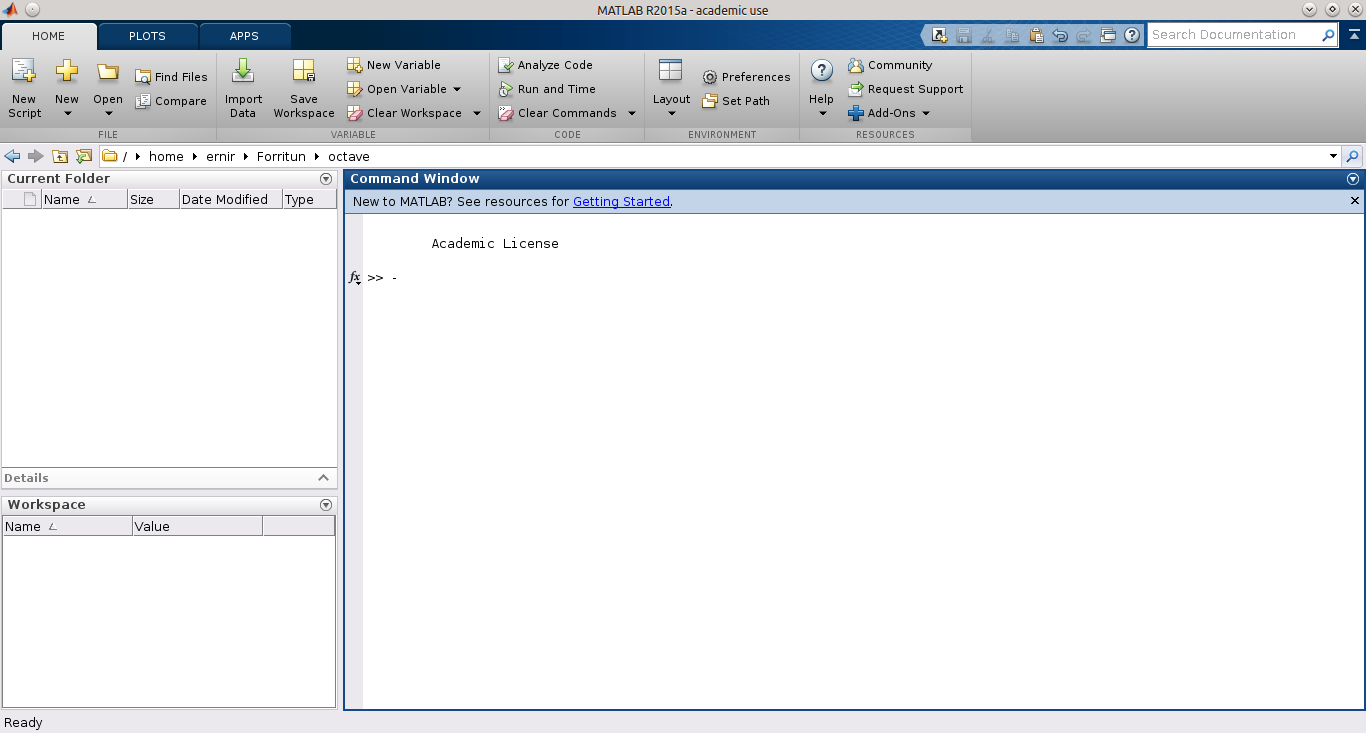
\includegraphics[width=\linewidth]{Pics/matlab-gui}
\end{frame}

\begin{frame}{Uppsetning Matlab}
\begin{itemize}
 \item Matlab er ekki ókeypis
 \begin{itemize}
  \item Fyrirtækið \emph{Mathworks Inc.} á Matlab
  \item Háskólinn býður upp á notkunarleyfi
  \item Uppsetningarleiðbeiningar má finna á: \url{https://notendur.hi.is/\~jonasson/matlab/}
 \end{itemize}
 \item Ókeypis og opið kerfi sem líkist Matlab er til, \href{https://www.gnu.org/software/octave/}{GNU Octave}
\end{itemize}
\end{frame}

\begin{frame}{Octave forritunarumhverfið}
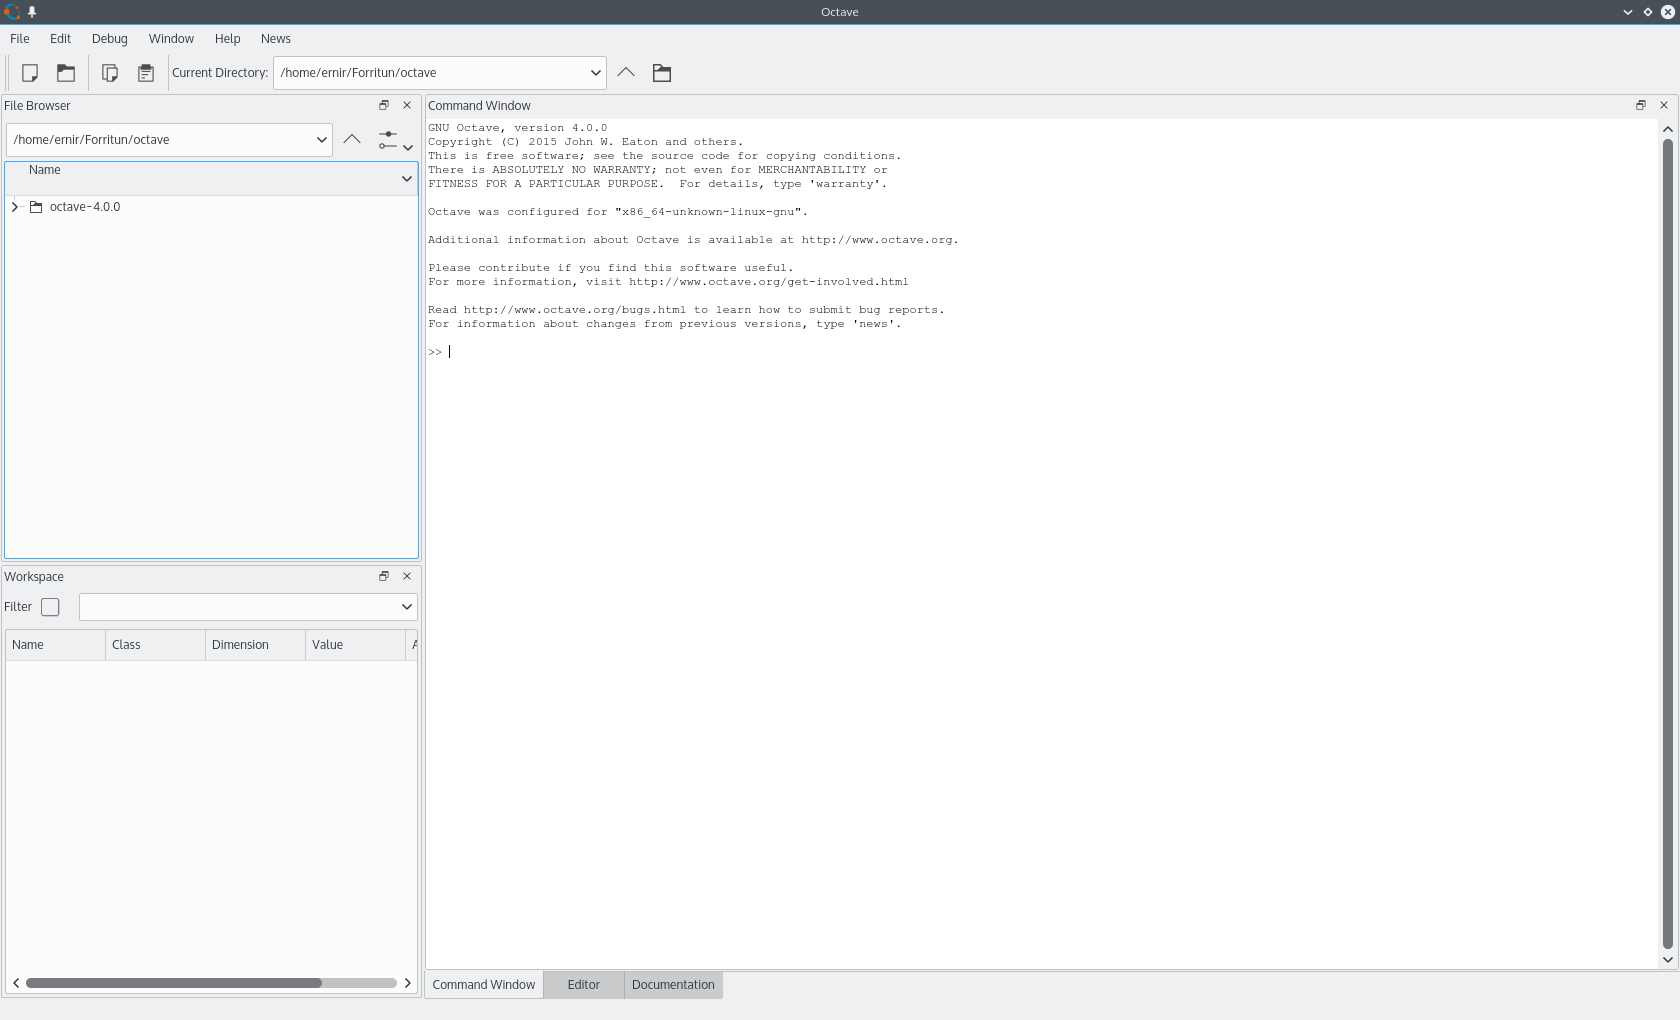
\includegraphics[width=\linewidth]{Pics/Octave4}
\end{frame}

\begin{frame}{Fyrirlestraræfing}
Skráið ykkur inn á \url{http://socrative.com/} og gerið fyrstu tvær spurningarnar.

Herbergisnúmer = \texttt{TOL105G2016}

Notendanafn = HÍ-tölvupóstfang
\end{frame}


\section{Bitar og tvíundartölur}

\begin{frame}{Bitar}
\begin{itemize} 
 \item Ef tölva er vél, þá er hún vél sem færir \emph{bita} á milli ástanda
 \item Líta má á bita sem ``hólf'' af upplýsingum - þar sem einu mögulegu upplýsingarnar eru í hvoru af tveimur ástöndum bitinn er
 \item \emph{Öll} gögn í tölvum eru geymd sem bitar
 \item Dæmi um einn bita af upplýsingum:
 \begin{itemize}
  \item ``Er spenna eða er ekki spenna á þessari rafrás?'' (örgjörvi)
  \item ``Snýr þessi segull norður/suður eða suður/norður?'' (harður diskur)
  \item ``Stutt eða langt?'' (morse-kóði)
 \end{itemize}
\end{itemize}
\end{frame}

\begin{frame}{Bæti}
\begin{itemize}
 \item Hópur af 8 bitum er kallaður bæti
 \item Minnishólf í tölvum eru heilt margfeldi af bætum
 \begin{itemize}
  \item Ekki er hægt að ná í einn bita í einu
  \item Bæti er minnsta nothæfa einingin
 \end{itemize}
\end{itemize}
\end{frame}

\begin{frame}{Merking bæta og bita?}

\begin{itemize}
 \item Hvað þýðir bætið 01001011? \pause
 \item Það er okkar að skilgreina.
 \begin{itemize}
  \item Gæti verið bókstafur
  \begin{itemize}
   \item samkv. ASCII er þetta 'K'
  \end{itemize}
   \item Gæti verið heiltala
  \begin{itemize}
   \item í tvíundarkerfinu er þetta 75
  \end{itemize}
  \item Gæti verið vélarmálsskipun (fer eftir örgjörva)
  \item Gæti verið hluti af kommutölu (eru 4 eða 8 bæti)
  \item Gæti verið hluti af mp3, jpeg eða mp4 skrá
 \end{itemize}
\end{itemize}
\end{frame}

\begin{frame}{Tvíundartölur}
\begin{itemize}
 \item Hvernig geymum við tugatölur (grunntala 10) með bitum (grunntala 2)? \pause
 \item Látum bitann í sæti $i$ tákna töluna $2^i$
 \item Dæmi:
\begin{align*}
1 		&=  2^0  	= 1\\
101		&=  2^2 + 2^0  =  4 + 1  =  5\\
01001011	&=  2^6 + 2^3 + 2^1 + 2^0  =  64 + 8 + 2 + 1 = 75
\end{align*}
\end{itemize}
\end{frame}

\begin{frame}{Áhugavert um tvíundartölur}
Það virkar að leggja saman tvíundartölur: 
\[
  00000001 + 00000010 = 00000011
\]
\[
 2^0 + 2^1 = 1 + 2 = 3
\]

Stærsta tvíundartala sem hægt er að tákna með einu bæti hlýtur þá að vera $11111111$, sem er talan $128+64+32+16+8+4+2+1$  $=  255$. Tilraunir til að vinna með stærri tölur en geymslusvæðið býður upp á veldur svokölluðu reikningsyfirflæði (e. \emph{overflow}).
\end{frame}

\begin{frame}{Neikvæðar tvíundartölur}
\begin{itemize}
 \item En hvernig má þá tákna neikvæðar tölur? \pause
 \item Algengast er að nota tvíandhverfu (e. \emph{Two's complement})
 \begin{itemize}
  \item Snúa öllum bitunum við og leggja 1 við
  \item Þá virkar venjuleg samlagning rétt áfram
 \end{itemize}
 \item Gerum ráð fyrir að tala sem er með 1 ``lengst til vinstri'' tákni neikvæða tölu
 \begin{itemize}
  \item Það bil jákvæðra talna sem kemst fyrir í minnishólfinu minnkar
 \end{itemize}
\end{itemize}
\end{frame}

\section{Breytur}

\begin{frame}{Breytur}
\begin{itemize}
 \item Gefum okkur að við höfum aðgang að minni í tölvu (samanstendur af bætum)
 \item Breyta (e. \emph{variable}) er afmarkað minnishólf sem inniheldur gildi
 \item Til að geta vísað í minnishólfið gefum við því nafn (breytuheiti, e. \emph{variable name})
 \item Stærð breyta er mismunandi eftir því hvaða af hvaða tagi (e. \emph{type} eða \emph{class}) gögnin eru
 \begin{itemize}
  \item Dæmi um tög eru heiltölur, fleytitölur, bókstafir, \ldots
 \end{itemize}
\end{itemize}
\end{frame}

\begin{frame}[fragile]{Að búa til breytur}
Dæmi um hvernig búa má til breytu:
\begin{minted}[frame=lines]{matlab}
>> myNumber = 6
myNumber =  
     6
\end{minted}
Merking skipunarinnar í efstu línunni er ``settu gildið $6$ í breytuna \texttt{myNumber}''. Matlab svarar með gildi nýju breytunnar.

Sé semíkomma sett á eftir skipuninni svarar Matlab ekki:
\begin{minted}[frame=lines]{matlab}
>> myNumber = 6;
\end{minted}
\end{frame}

\begin{frame}{Workspace-glugginn}
\begin{columns}
\column{0.5\textwidth}
\begin{itemize}
 \item Workspace-glugginn sýnir ýmsar upplýsingar um skilgreindar breytur
 \item Hægri-smella má á dálkana til að sýna fleiri
\end{itemize}
\column{0.5\textwidth}
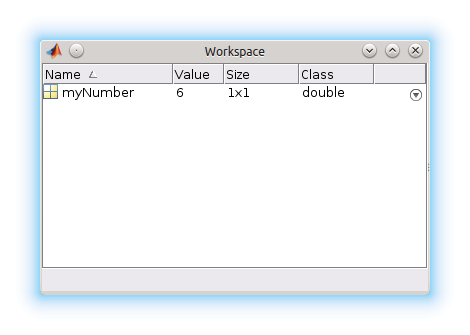
\includegraphics[width=\linewidth]{Pics/workspace-window}
\end{columns}
\end{frame}

\begin{frame}[fragile]{Breytan \texttt{ans}}
Breytan \texttt{ans} er sjálfkrafa gefið gildi þegar reiknisetning er framkvæmd 
\begin{minted}[frame=lines]{matlab}
>> 2+3
ans = 
     5
\end{minted}
\end{frame}

\begin{frame}[fragile]{Að nota breytur}
Breytur geymast, svo hægt er að nota þær áfram (annars væri lítið gagn í þeim)
\begin{minted}[frame=lines]{matlab}
>> x = 1;
>> y = 2;
>> x + y
ans =
     3
\end{minted}
Breyta helst skilgreind þar til henni er eytt eða þar til við förum út úr sviði (e. \emph{scope}) breytunnar (meira síðar)
\end{frame}

\begin{frame}{Breytuheiti}
\begin{itemize}
 \item Allar breytur hafa nöfn
 \begin{itemize}
  \item Nöfnin verða að byrja á bókstaf (úr stafrófinu)
  \begin{itemize}
   \item \texttt{number123} er í lagi, en  \texttt{123number}  ekki í lagi
   \item Breytuheiti mega ekki innihalda bil
  \end{itemize}
  \item Engir séríslenskir stafir leyfðir
  \begin{itemize}
   \item \texttt{upphaed}  er í lagi, en  \texttt{upphæð}  ekki í lagi
  \end{itemize}
  \item Greinarmunur gerður á hástaf og lágstaf
  \begin{itemize}
   \item \texttt{mynumber}, \texttt{Mynumber} og \texttt{MYNUMBER} eru allt aðskildar breytur
   \item Tillaga: Láta breytuheiti byrja á litlum staf, nota hástafi til að skilja á milli orða: \texttt{myNumber}
  \end{itemize}
  \item Nokkur lykilorð (key words) eru frátekin af Matlab og má ekki nota sem nöfn
  \begin{itemize}
   \item \texttt{>> if = 4;}    gefur villu
  \end{itemize}
 \end{itemize}
\end{itemize}
\end{frame}

\begin{frame}[fragile]{Meira um breytuheiti}
\begin{itemize}
 \item Reynum að hafa breytuheiti lýsandi
 \begin{itemize}
  \item \texttt{force = mass * acceleration} er skýrara en \texttt{z = x * y} 
 \end{itemize}
 \item Það að breytuheiti sé löglegt þýðir ekki endilega að það sé \emph{gott}
 \begin{itemize}
  \item T.d. er hægt að yfirskrifa innbyggðar breytur:
\begin{minted}[frame=lines]{matlab}
>> pi = 4;
>> radius = 2;
>> area = radius^2 * pi
area = 
      16
\end{minted}
 \end{itemize}
\end{itemize}
\end{frame}

\begin{frame}{Skipanir tengdar breytum}
\begin{center}
\begin{tabular}{ll}
\toprule
Skipun&Merking\\
\midrule
\texttt{who}&sýnir nöfn skilgreindra breyta\\
\texttt{whos}&sýnir upplýsingar um breytur\\
\texttt{clear}&eyðir öllum skilgreindum breytum\\
\texttt{clear <breyta>}&eyðir tiltekinni breytu\\
\bottomrule
\end{tabular}
\end{center}
\end{frame}

\begin{frame}{Tög breyta}
\begin{itemize}
 \item Allar breytur hafa tag
 \item Matlab ákvarðar tag breytu sjálfkrafa út frá gildinu sem breytunni er gefið
 \item Helstu tög eru:
 \begin{itemize}
  \item Kommutölur (e. \emph{floating point numbers}):  \texttt{single}, \texttt{double}
  \begin{itemize}
   \item \texttt{double} er sjálfgefna tagið fyrir tölur
  \end{itemize}
  \item Heiltölur (e. \emph{integers}): \texttt{int8}, \texttt{int16}, \texttt{int32}, \texttt{int64}
  \item Bókstafir (e. \emph{characters}): \texttt{char}
  \begin{itemize}
   \item T.d. \texttt{'a'} og \texttt{'halló heimur'}
  \end{itemize}
  \item Rökgildi (e. \emph{logical} eða \emph{boolean}): \texttt{logical}
  \begin{itemize}
   \item Bara tvö möguleg gildi: \texttt{true} og \texttt{false} (eða 1 og 0)
  \end{itemize}
 \end{itemize}
\end{itemize}
\end{frame}

\begin{frame}{Fyrirlestraræfing}
Skráið ykkur inn á \url{http://socrative.com/} og klárið æfinguna.

Herbergisnúmer = \texttt{TOL105G2016}

Notendanafn = HÍ-tölvupóstfang
\end{frame}

\end{document}
